\documentclass[border=8pt]{standalone}
\usepackage{libertine}
\usepackage{amsmath,amssymb}
\usepackage{tikz}
\begin{document}
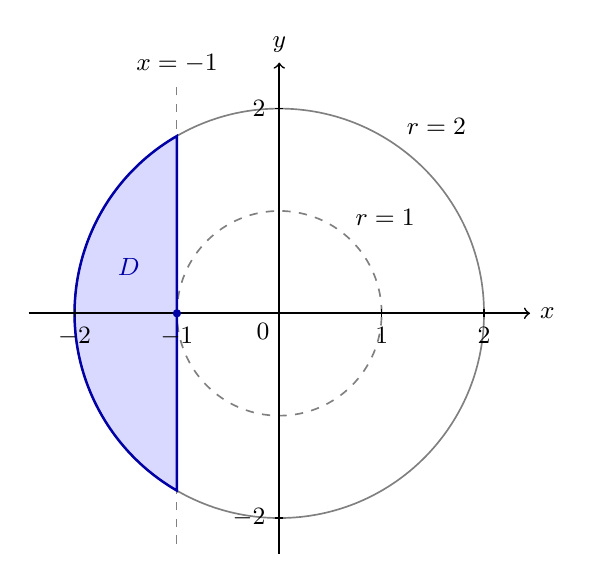
\begin{tikzpicture}[x=1.3cm,y=1.3cm,font=\small]
  % Annulus 1 <= r <= 2, restricted to -2 <= x <= -1.
  % The unit circle touches this retained cap only at (-1,0).
  \fill[blue!15] (-1,{sqrt(3)})
    arc[start angle=120,end angle=240,radius=2]--cycle;
  \draw[gray,line width=0.6pt] (0,0) circle (2);
  \draw[gray,dashed,line width=0.6pt] (0,0) circle (1);
  \draw[gray,dashed] (-1,-2.25)--(-1,2.25) node[above,black] {$x=-1$};
  \draw[blue!65!black,line width=0.9pt] (-1,{sqrt(3)})
    arc[start angle=120,end angle=240,radius=2]--cycle;
  \draw[->,line width=0.6pt] (-2.45,0)--(2.45,0) node[right] {$x$};
  \draw[->,line width=0.6pt] (0,-2.35)--(0,2.45) node[above] {$y$};
  \foreach \a in {-2,-1,1,2} {
    \draw (\a,0.04)--(\a,-0.04) node[below] {$\a$};
  }
  \foreach \b in {-2,2} {
    \draw (0.04,\b)--(-0.04,\b) node[left] {$\b$};
  }
  \node[below left] at (0,0) {$0$};
  \node[above right] at (1.15,1.65) {$r=2$};
  \node[above right] at (0.65,0.76) {$r=1$};
  \node[blue!65!black] at (-1.47,0.45) {$D$};
  \fill[blue!65!black] (-1,0) circle (1.5pt);
\end{tikzpicture}
\end{document}
